\pdfoutput=1
\documentclass[12pt]{article}

\usepackage[T1]{fontenc}
\usepackage{lmodern}
\usepackage{amsmath,amssymb}
\usepackage{graphicx}
\usepackage{booktabs}
\usepackage{longtable}
\usepackage[margin=1in]{geometry}
\linespread{1.15}
\usepackage[font=small,labelfont=bf]{caption}
\usepackage{microtype}
\usepackage{natbib}
\usepackage[hyphens]{url}
\Urlmuskip=0mu plus 1mu\relax
\usepackage[hidelinks,breaklinks]{hyperref}
\emergencystretch=1.5em

\newcommand{\unit}[1]{\,\mathrm{#1}}
\newcommand{\degree}{\ensuremath{{}^\circ}}

\title{Atmospheric Model Response and Conditional Orbital Consequences of the February 2022 Starlink Deployment}
\author{Onur A. W. Aydogan\\\small Waynestark Enterprises Limited}
\date{24 November 2026}

\begin{document}
\maketitle

\begin{abstract}
Geomagnetic disturbances during low-perigee satellite deployments increase thermospheric density and accelerate orbital decay, yet quantifying storm-attributable loss without telemetry requires separating forward model sensitivity from observational reconstruction. Here we evaluate fixed-point and path-integrated thermospheric responses alongside paired quiet-versus-storm propagations for the February 2022 Starlink Group~4-7 deployment. At $210\unit{km}$, $53.22\degree$\,N, $0\degree$\,E, NRLMSISE-00, NRLMSIS~2.0 and NRLMSIS~2.1 yield actual-to-quiet peak enhancements of $17.14\,\%$ to $18.77\,\%$ against a constant $ap=4$ counterfactual, while sweeping $ap=2$ to $7$ moves NRLMSISE-00 from $20.58\,\%$ to $13.18\,\%$. Across $200$--$300\unit{km}$, fixed-point WAM-IPE to NRLMSISE-00 ratios of independently maximised peak percentage enhancements span $2.84$--$5.40$ under same-UTC-hour reference days versus $1.12$--$1.62$ under whole-day means. These compare non-simultaneous percentage peaks rather than absolute densities: at $210\unit{km}$ on the 1~February same-UTC-hour baseline, the $53.49\,\%$ WAM-IPE and $17.17\,\%$ NRLMSISE-00 peaks occur $2\unit{h}$ apart, versus a $1.60$ median matched-hour density ratio. Along the $96\unit{h}$ planned orbit, WAM-IPE increases path-integrated orbital-energy loss by $49.5\,\%$ ($48.4\,\%$ over contiguous non-gap segments). Under NRLMSIS~2.1 with legacy centroid shadowing, observed drivers advance $170\unit{km}$ crossings by $5.94\unit{h}$ ($11.77\,\%$) at $30\degree$, $3.04\unit{h}$ ($10.25\,\%$) broadside and $29.71\unit{h}$ ($6.69\,\%$) edge-on. Replacing centroid masking (which jumps $+14.45\,\%$ off $0\degree$) with continuous collimated-area or parallel-plate kinetic cavity shadowing in NRLMSISE-00 shortens edge-on crossings by $15.1\,\%$--$15.8\,\%$ (advance $26.79\unit{h}$ to $25.28\unit{h}$) and shifts $30\degree$ advance from $5.93\unit{h}$ to $5.95\unit{h}$. All contrasts remain conditional model properties rather than observed satellite lifetimes.
\end{abstract}

\noindent\textbf{Keywords:} thermospheric mass density, geomagnetic storm response, low-Earth-orbit drag, Starlink Group 4-7, counterfactual orbital propagation, free-molecular aerodynamics

\section{Introduction}
\label{sec:intro}

Very-low-altitude satellite deployments pass through a region of the upper atmosphere where modest geomagnetic activity produces immediate operational consequences. When SpaceX launched the forty-nine Starlink Group~4-7 spacecraft into an elliptical staging orbit near $210\unit{km}$ perigee on 3~February 2022 during moderate geomagnetic storm conditions, thirty-eight spacecraft eventually re-entered and thirty-two were never catalogued by space-surveillance tracking. The recorded launch outcome motivates an orbital sensitivity calculation but does not specify the histories needed to reconstruct individual losses \citep{guarnieri2025}. In the absence of public spacecraft state vectors at release, attitude histories, thruster firings or onboard drag telemetry, forward orbital calculations must distinguish strictly between conditional model behaviour under declared counterfactual inputs and empirical reconstruction of the actual fleet loss.

Two distinct scientific questions govern forward modelling of this event. First, how strongly do empirical MSIS-family thermospheric models respond at staging altitude relative to their own quiet-driver baselines and relative to archived physics-based operational forecasts across same-UTC-hour and whole-day-mean reference operators, and what prevents direct numerical ranking against published event anomalies? Second, when a facet-resolved, species-resolved free-molecular force model is integrated forward from a planned insertion state under paired quiet and observed geomagnetic histories, how much earlier does the observed-driver trajectory cross a declared free-molecular threshold altitude across prescribed spacecraft attitudes, and how sensitive are those crossing times to non-convex panel-shadowing approximations and path-local rarefaction bounds?

Answering those questions cleanly requires separating forward atmospheric--orbital sensitivity from two companion problems treated in parallel articles of this three-paper portfolio. The inverse calibration problem --- what public satellite-catalogue decay dates can and cannot identify when atmospheric density scale and spacecraft drag enter as a product across a mixed payload-and-debris sample --- is developed in Companion Paper~II. The microscopic aerodynamic problem --- how gas species, facet incidence, exact kinetic thermal-cavity shadowing, diffuse versus Cercignani--Lampis--Lord scattering kernels, and Langmuir accommodation govern free-molecular forces on the eight-facet spacecraft proxy --- is established in Companion Paper~III. All three articles share one frozen computational archive and partition a single body of evidence into three distinct scientific questions rather than claiming independent experimental replications.

Four methodological boundaries govern every result in this article. First, the three empirical atmosphere configurations (NRLMSISE-00, NRLMSIS~2.0 and NRLMSIS~2.1) belong to one model lineage driven by identical solar and geomagnetic indices; agreement among them reflects internal family consistency rather than a bound on real thermospheric error. Second, storm-time percentage enhancements depend strongly on whether anomalies are formed against a constant-$ap$ counterfactual, same-UTC-hour reference-day profiles or whole-day reference means. Published atmospheric studies use different altitude, averaging and reference conventions \citep{fang2022,he2023}. Third, the paired orbital runs report elapsed time from deployment to the first descending crossing of $170\unit{km}$ instantaneous geodetic altitude rather than observed re-entry lifetimes, and we explicitly test how binary centroid shadowing versus continuous collimated and kinetic cavity shadowing alters both edge-on and inclined trajectories. Fourth, fixed-point density ratios, single-state force offsets, attitude scenario spans and integrated crossing-time advances concern different observables, operators, baselines and denominators; they are reported side by side without causal ranking.

Section~\ref{sec:literature} examines prior thermospheric modelling studies of the February 2022 storm and establishes the formal operator mismatch that precludes a direct literature ranking table. Section~\ref{sec:methods} defines the deployment specification, geomagnetic counterfactuals, density conventions, WAM-IPE interpolation and baseline operators, translational equations of motion, moving attitude frame and Knudsen cutoff. Section~\ref{sec:results} presents the atmospheric comparisons, path-energy integrals and paired orbital propagations across visibility models. Section~\ref{sec:discussion} synthesises the findings and physical limitations, Section~\ref{sec:conclusions} states the conclusions, and Section~\ref{sec:availability} summarises code and data availability.

\section{Literature Context and Research Gap}
\label{sec:literature}

\subsection{Prior thermospheric modelling of the February 2022 storm}
\label{sec:prior-storm}

Two primary modelling studies in the space-weather literature examine neutral-density enhancements during the 3--4~February 2022 geomagnetic storm: Fang et~al.\ (2022), who compare operational Whole Atmosphere Model--Ionosphere Plasmasphere Electrodynamics (WAM-IPE, written WAM in their notation) simulations against empirical thermospheric models and an onboard Starlink drag proxy, and He et~al.\ (2023), who evaluate empirical and physics-based thermospheric models against Swarm-A, GRACE-FO and GOLD observations across storm phases. Both studies examine NRLMSIS~2.0, while Fang et~al.\ additionally evaluate NRLMSISE-00 and DTM2020 and He et~al.\ evaluate DTM2013, CTIPe, MAGE, WAM-IPE and SD-WACCMX. Neither study evaluates NRLMSIS~2.1 directly.

Fang et~al.\ (2022) report a substantial contrast between WAM-IPE and empirical models during the event. At $210\unit{km}$ at 11:50~UT on 4~February, relative to ten-day-averaged densities from each model at the same universal time, WAM-IPE indicates at least a $50\,\%$ density increase across most regions and more than $100\,\%$ in localised areas, whereas MSIS-00 shows only up to $20\,\%$. Across $200$ to $400\unit{km}$, their WAM-IPE simulations yield enhancements of $50$--$125\,\%$. Along the orbits of two Starlink satellites, they report WAM-IPE absolute densities roughly $40$--$80\,\%$ higher than MSIS-00 at perigees and $60$--$100\,\%$ higher at apogees, with larger perigee changes from 4 to 7~February; adding MSIS~v2.0 and DTM2020 along those orbits, they find WAM-IPE absolute densities larger than all three empirical models, MSIS~v2.0 slightly higher than MSIS-00, and both MSIS models higher than DTM2020. For storm anomalies not plotted, they note an MSIS~v2.0 enhancement up to $50\,\%$ alongside no pronounced enhancement in MSIS-00 or DTM2020, and note that pre-launch Starlink Monte Carlo analyses using MSIS-00 expected roughly a $50\,\%$ density increase, which was approximately the level required to initiate satellite safehold.

He et~al.\ (2023) resolve the event by storm phase and altitude, finding positive or negative model biases depending on storm phase. Against Swarm-A orbit-averaged relative changes near $438\unit{km}$, they find DTM2013, CTIPe, MAGE and WAM-IPE consistent with the 3~February increase while MSIS~2.0 and SD-WACCMX underestimate it by about $50\,\%$. On 4~February, CTIPe lies closest to Swarm-A, DTM2013 and WAM-IPE underestimate the relative increase by about $30\,\%$, MSIS~2.0 and SD-WACCMX underestimate by about $50$--$70\,\%$, and MAGE overestimates by about $10\,\%$. During 5~February recovery, DTM2013, MSIS~2.0, WAM-IPE and SD-WACCMX agree closely with Swarm-A while CTIPe and MAGE overestimate by about $30\,\%$, and on 6~February WAM-IPE and MAGE underestimate by about $20\,\%$. In absolute density against Swarm-A, MSIS~2.0 underestimates during 3--4~February, DTM2013 overestimates on 2 and 5--6~February, MAGE overestimates 4~February by about $50\,\%$ in amplitude and $12\unit{h}$ in duration, and WAM-IPE overestimates in both quiet and disturbed intervals. Against GRACE-FO near $505\unit{km}$, CTIPe and MAGE agree best with observed densities while WAM-IPE underestimates enhancements on 3--4~February, with inter-model discrepancies reaching $70\,\%$.

In an orbital-drag study of the same February 2022 event, \citet{baruah2024} coupled JB2008 thermospheric densities with an assumed $1\unit{m^2}$ ram-area drag approximation and reported approximately six hours of storm-accelerated decay under their timing definition. Our contribution is therefore not a claim that a six-hour figure is novel in isolation, but rather quantifying how the modelled $170\unit{km}$ threshold-crossing advance varies strongly with prescribed attitude ($3.04$--$29.71\unit{h}$ across $90\degree$, $30\degree$ and $0\degree$ under NRLMSIS~2.1), atmospheric reference operator, and continuous versus kinetic panel-shadowing treatment, while establishing explicitly that conditional forward simulations do not identify the decay duration of any individual flown satellite.

Complementing these thermospheric modelling studies, \citet{nager2026} examine operational space-weather decision frameworks for proactive small-satellite constellation risk classification during geomagnetic disturbances (HELIO), a forecast-to-action operational question distinct from the forward atmospheric-model and orbital-propagation sensitivity quantified here.

\subsection{Definitional non-comparability and observational altitude bounds}
\label{sec:nolitcompare}

Despite studying the same geomagnetic storm, placing fixed-point counterfactual enhancement percentages into a direct numerical ranking table against published figures is precluded by mathematical operator mismatch. Meaningful numerical comparison requires matching the evaluation altitude, spatial-temporal averaging operator and quiet reference baseline simultaneously. Our primary empirical metric evaluates a temporal peak at one fixed coordinate ($210\unit{km}$, $53.22\degree$\,N, $0\degree$\,E) against a counterfactual holding $ap=4$ at observed solar flux. By contrast, published metrics evaluate spatial fields or zonal means against multi-day averages or calendar reference days. Fang et al.'s printed page~7 describes a $210\unit{km}$ comparison at 11:50~UT on 4~February against a ten-day model mean \citep{fang2022}. He et al.'s printed page~15 (PDF page~16) describes zonal-mean $200\unit{km}$ enhancements against 1--2~February references \citep{he2023}. Neither operator bounds a fixed-point temporal peak, and Fang et~al.'s MSIS-00 figure (``up to $20\,\%$'') states a spatial ceiling rather than a target interval.

Even under one study's conventions, enhancements near staging altitudes do not partition cleanly by model family. The enhancement values that He et al.\ report at $200\unit{km}$ do not order the models by family: they report enhancements of up to about $30$--$35\,\%$ for DTM2013 on both 3 and 4~February, about $10$--$15\,\%$ for MSIS~2.0 during the two storm days, and about $20\,\%$ on 3~February and $30\,\%$ on 4~February for CTIPe. For the remaining models at $200\unit{km}$, they report about $30\,\%$ on 3~February (in the middle and low latitudes) and $40\,\%$ on 4~February for MAGE, about $10$--$15\,\%$ on 3--4~February for WAM-IPE, and about $10\,\%$ on 4~February for SD-WACCMX \citep[p.~15]{he2023}. At $300\unit{km}$, He et~al.\ report global-averaged maxima on 3 and 4~February of $50\,\%$ and $45\,\%$ for DTM2013, $20\,\%$ and $25\,\%$ for MSIS~2.0, $41\,\%$ and $51\,\%$ for CTIPe, $57\,\%$ and $75\,\%$ for MAGE, $40\,\%$ and $40\,\%$ for WAM-IPE, and $15\,\%$ and $23\,\%$ for SD-WACCMX (with CTIPe--MAGE averages near $35\,\%$ at $200\unit{km}$ and $60\,\%$ at $300\unit{km}$).

Direct observational certification of neutral density at $210\unit{km}$ is likewise absent from these sources: the abstract of \citet{he2023} records Swarm-A at about
$438\unit{km}$ and GRACE-FO at about $505\unit{km}$, against $210\unit{km}$ here, more than two hundred kilometres above staging perigee, while Fang et~al.'s onboard Starlink drag-over-$C_D$ proxy across $200$--$250\unit{km}$ depends on unverified onboard drag coefficients. Quantifying same-point baseline operator sensitivity at $210\unit{km}$ alongside propagated threshold-crossing sensitivity across explicit panel-visibility formulations therefore addresses a concrete gap.

\section{Methodology and Atmospheric--Orbital Framework}
\label{sec:methods}

\subsection{Evaluation modes and event deployment conventions}
\label{sec:data}

Every calculation in this article operates in one of three distinct computational modes. Fixed-point atmospheric evaluations hold geographic coordinates fixed at $210\unit{km}$ geodetic altitude, $53.22\degree$\,N latitude and $0\degree$\,E longitude across 145 hourly samples spanning $144\unit{h}$ from 2022-02-02 00:00~UTC to 2022-02-08 00:00~UTC. Single-state aerodynamic diagnostics evaluate forces at one frozen thermospheric state and relative speed ($7495.2\unit{m\,s^{-1}}$ at 2022-02-04 14:00~UTC). Propagated orbital experiments integrate three translational degrees of freedom (six first-order Cartesian state equations) forward from a common planned release state under paired geomagnetic histories until the trajectory first crosses a selected geodetic altitude threshold.

Guarnieri et al.'s 2023 preprint reports that Group~4-7 (COSPAR designator 2022-010) launched at 2022-02-03T18:13Z and released its spacecraft 15~min~31~s later, at 18:28Z. It describes an \emph{initial planned} elliptical orbit of $338\times210\unit{km}$ at $53.22\degree$ inclination and an intended operational altitude of approximately $540\unit{km}$ \citep[\S2]{guarnieri2023v1}. Its abstract reports 49 released spacecraft, 38 eventually lost and 32 never tracked. The preprint treats immediate loss of those 32 as an assumption and also discusses tracking-position problems; absence of tracking therefore does not establish their loss times \citep[\S4]{guarnieri2023v1}. The later journal edition also states an operational altitude of approximately $540\unit{km}$ \citep[p.~76]{guarnieri2025}.

Our propagations adopt the minute-precision release epoch \texttt{2022-02-03T18:28:00Z}. Adding $15\unit{min}\ 31\unit{s}$ to an unrounded liftoff within \texttt{18:13Z} places actual release between roughly $1\unit{s}$ and under $60\unit{s}$ after \texttt{18:28:00Z} under readings consistent with both stated minutes (or under $91\unit{s}$ if the \texttt{18:28Z} minute is not treated as an independent constraint), comparable to the $0.01\unit{h}$ ($36\unit{s}$) reporting precision of Table~\ref{tab:lifetimes}; no shifted-epoch facet-resolved paired propagation was executed. Because no individual spacecraft insertion state is publicly available, perigee is placed on the inertial $+x$ axis with right ascension of the ascending node, argument of perigee and initial true anomaly all set to zero as an explicit convention.

\subsection{Geomagnetic drivers and quiet counterfactual definition}
\label{sec:quiet}

Geomagnetic $ap$ comes from the GFZ $K_p/ap$ series \citep{gfzkp} and solar
$F_{10.7}$ and $F_{10.7a}$ from the CelesTrak daily space-weather file
\citep{celestrak}. Extended 1~January--31~May 2022 three-hourly GFZ payloads drive all atmosphere and trajectory integrations. Each MSIS evaluation receives the standard seven-element storm-mode $ap$ history vector (UTC calendar-day daily $Ap$ averaged over the eight three-hourly indices of the calendar day --- e.g.\ $Ap = 32.0$ on 4~February 2022 --- followed by the current three-hour $ap$, three preceding three-hour values, and two eight-step averages covering $12$--$33\unit{h}$ and $36$--$57\unit{h}$ prior). The storm-time activity switch is set to $-1$, alongside preceding-day observed $F_{10.7}$ and the 81-day centred mean $F_{10.7a}$. At the $210\unit{km}$ peak-enhancement instant (2022-02-04 20:00~UTC), switching from daily-$Ap$ mode ($Ap = 32.0$) to storm-time mode increases NRLMSISE-00 mass density by $+2.53\,\%$ ($+2.532\,\%$; $+2.62\,\%$ in NRLMSIS~2.0 and~2.1). Direct verification across all $145$ window hours and across $100$--$338\unit{km}$ confirms exact $0.000\times10^{0}$ bit-level invariance of storm-mode ($sw_9 = -1$) NRLMSISE-00, NRLMSIS~2.0 and NRLMSIS~2.1 densities, temperatures and species concentrations (including NO) to the first array slot $Ap$.

The baseline ``quiet'' counterfactual replaces every entry of the seven-element $ap$ vector with $ap=4$ ($K_p = 1\mathrm{o}$) while holding $F_{10.7}$ and $F_{10.7a}$ at their observed trajectories. To quantify sensitivity to this baseline definition, a one-at-a-time sweep on the NRLMSISE-00 species-sum branch evaluates $ap \in \{0, 2, 4, 7, 12\}$ at the $ap=4$ enhancement-peak instant (2022-02-04 20:00~UTC), yielding enhancements of $24.91\,\%$, $20.58\,\%$, $17.14\,\%$, $13.18\,\%$ and $8.68\,\%$ (with window peaks over $ap=2$ to $7$ spanning $20.58\,\%$ to $13.18\,\%$, corresponding to $K_p = 0.333$ [$0+$] through $K_p = 2.000$ [$2\mathrm{o}$] across all 313 three-hourly GFZ records; native-total and species-sum $ap=4$ peaks are $0.1714295$ and $0.1714296$). No quiet-$ap$ sweep was executed for NRLMSIS~2.0 or~2.1.

\subsection{Empirical atmosphere models and density conventions}
\label{sec:densities}

NRLMSISE-00 \citep{picone2002} is evaluated through the \texttt{pymsis} package;
NRLMSIS~2.0 \citep{emmert2021} and~2.1 through a Fortran driver built against the
official NRL source, which is not redistributed with this work. As documented by Emmert et~al.\ (2022)\nocite{emmert2022}, NRLMSIS~2.1 upgrades NRLMSIS~2.0 solely by adding nitric oxide (NO) number density while retaining the NRLMSIS~2.0 temperature and major-species parameterisations.

Two mass-density definitions are distinguished throughout. First, the \emph{native model total} is the aggregate mass density returned directly by each model; all fixed-point peaks and inter-model ratios in Table~\ref{tab:atmos} use this native output. In the official NRLMSIS~2.1 Fortran source (\texttt{msis\_init.F90}), NO is added as species index~10 with zero mass weight (\texttt{masswgt(10) = 0.0\_rp}), excluding NO from native total density so that native NRLMSIS~2.1 and~2.0 totals match to double-precision rounding by construction. Second, the \emph{species sum} $\rho = \sum_j m_j n_j$ sums per-species number densities multiplied by integer mass numbers times the atomic mass constant ($1.6605390666\times10^{-27}\unit{kg}$), including NO ($4.61\times10^{-2}\,\%$ of species-sum mass at 2022-02-04 14:00~UTC). Every species-resolved force evaluation uses this species sum and normalises $C_D = D/(\tfrac12 \rho V_{\mathrm{rel}}^2 A_{\mathrm{ref}})$ by it. Because NRLMSIS~2.1 uses CIPM~2007 molar masses ($28.0134$ versus $28$ for $\mathrm{N_2}$), integer mass numbers shift $\rho$ by $-2.34\times10^{-2}\,\%$ and unshadowed single-state drag by $-2.29\times10^{-2}\,\%$ (ratio $0.979$), combining with NO inclusion to leave a $+2.27\times10^{-2}\,\%$ species-versus-native closure gap (Companion Paper~III).

\subsection{Archived WAM-IPE field, baseline operators and path-energy integrals}
\label{sec:wam}

The comparison density field is the CCMC external-run archive of the SWPC WAM-IPE Forecast System operational run, labelled July2021--22, using the fixed-height postprocessed \nolinkurl{wam_fixed_height.gsm10} NetCDF product \citep{ccmcwamipe}. The local archive holds 180 hourly NetCDF slices from 2022-02-01 00:00~UTC to 2022-02-08 23:00~UTC; six hourly files (10:00--15:00~UTC) are absent on both 5 and 7~February, leaving 133 of the 145 hourly samples inside the 2--8~February window. Neutral mass density \texttt{den} ($\mathrm{kg\,m^{-3}}$) on fixed height levels \texttt{hlevs} ($\mathrm{km}$) is sampled using mixed spatial-temporal interpolation: linear in $\ln\rho$ with altitude between bounding height levels, bilinear in $\rho$ across latitude and longitude, and linear in universal time between bracketing hourly slices (refusing evaluation whenever a slice gap exceeds one hour).

Because the CCMC archive contains a single operational forecast without an $ap=4$ counterpart, we evaluate WAM-IPE against NRLMSISE-00 using identical operators on both models. First, across all $N=180$ overlapping archive hours (1--8~February), we compute hourly absolute density ratios $\rho_{\mathrm{WAM}}(t)/\rho_{\mathrm{MSIS}}(t)$ (and over the 133 window hours against both NRLMSISE-00 and NRLMSIS~2.1). Second, for each candidate archive reference day $d_{\mathrm{ref}} \in \{\text{1~Feb, 2~Feb, 8~Feb}\}$ (retaining $N = 180 - 24 = 156$ non-reference evaluation hours $t \notin d_{\mathrm{ref}}$), we evaluate and contrast two distinct baseline operators explicitly:
\begin{equation}
\Delta_{\mathrm{sh}}(t; d_{\mathrm{ref}})
  = \frac{\rho(t)}{\rho\bigl(d_{\mathrm{ref}}, h_{\mathrm{UTC}}(t)\bigr)} - 1,
\qquad
\Delta_{\mathrm{dm}}(t; d_{\mathrm{ref}})
  = \frac{\rho(t)}{\frac{1}{24}\sum_{h=0}^{23}\rho(d_{\mathrm{ref}}, h)} - 1.
\label{eq:wam-operators}
\end{equation}
Here $\Delta_{\mathrm{sh}}$ is the \emph{same-UTC-hour} reference-day anomaly operator, which divides each hour $t$ by the density at the identical universal-time hour $h_{\mathrm{UTC}}(t)$ on $d_{\mathrm{ref}}$ to suppress the background diurnal tide, whereas $\Delta_{\mathrm{dm}}$ divides by the 24-hour calendar-day mean $\bar{\rho}(d_{\mathrm{ref}})$. Note that 1~February is not quiet at $ap=4$ (its eight three-hourly UTC calendar-day $ap$ values are $6, 6, 3, 3, 5, 3, 2, 18$, averaging $5.75$ and spanning $2$--$18$).

Third, along a drag-free two-body-plus-$J_2$ propagation of the planned orbit over $96\unit{h}$ from 2022-02-03 18:28~UTC to 2022-02-07 18:28~UTC at $300\unit{s}$ ($5\unit{min}$) steps ($1\,153$ grid instants), $168$ instants fall inside two $425\unit{min}$ ($7\unit{h}\ 05\unit{min}$) WAM-IPE archive gaps (\texttt{2022-02-05 08:58--16:03 UTC} across altitudes $294.8$--$322.8\unit{km}$, and \texttt{2022-02-07 08:58--16:03 UTC} across $275.5$--$326.5\unit{km}$), leaving $985$ valid samples across three contiguous sub-intervals ($463$, $492$ and $30$ samples). With scalar drag acceleration $\mathbf{a}_D = -\tfrac12 \rho \gamma |\mathbf{v}_{\mathrm{rel}}|\mathbf{v}_{\mathrm{rel}}$ at fixed $\gamma = 0.026246\unit{m^2\,kg^{-1}}$ (which cancels from all cross-model and storm-to-quiet ratios), we evaluate both the magnitude of specific inertial orbital-energy change $\Delta E_{\mathrm{orb}} = \bigl|\int \mathbf{a}_D\cdot\mathbf{v}\,\mathrm{d}t\bigr|$ (the primary stored path metric) and specific atmosphere-relative dissipation $E_{\mathrm{diss}} = \int (-\mathbf{a}_D\cdot\mathbf{v}_{\mathrm{rel}})\,\mathrm{d}t = \int \tfrac12\rho\gamma V_{\mathrm{rel}}^3\,\mathrm{d}t$, reporting both the historical $985$-point quadrature (which bridges the two gaps with single trapezoids omitting roughly five interior perigee passes each) and the exact sum over the three contiguous non-gap segments.

\subsection{Translational dynamics, moving attitude frame and energy-rate identity}
\label{sec:frames}

Orbital trajectories integrate the Cowell initial-value problem in an Earth-centred inertial (ECI) Cartesian frame $(\mathbf{r}, \mathbf{v}) \in \mathbb{R}^6$ (precession, nutation and polar motion omitted over multi-day decay arcs):
\begin{equation}
\dot{\mathbf{r}} = \mathbf{v},\qquad
\dot{\mathbf{v}} = -\frac{\mu}{r^3}\mathbf{r} + \mathbf{a}_{J_2}(\mathbf{r}) + \frac{\mathbf{F}_{\mathrm{aero}}(\mathbf{r},\mathbf{v},t)}{m},
\label{eq:cowell}
\end{equation}
where $r = |\mathbf{r}|$, $\mu = 3.986004418\times10^{14}\unit{m^3\,s^{-2}}$, WGS-84 equatorial radius $R_e = 6\,378\,137\unit{m}$, flattening $f = 1/298.257223563$ (geodetic altitude and latitude via Bowring's method; Greenwich sidereal time via IAU~1982), $J_2 = 1.08262668\times10^{-3}$, and
\begin{equation}
\mathbf{a}_{J_2}(\mathbf{r})
  = \frac{3}{2}\frac{J_2 \mu R_e^2}{r^5}
    \begin{pmatrix}
      x\bigl(5 z^2/r^2 - 1\bigr) \\[2pt]
      y\bigl(5 z^2/r^2 - 1\bigr) \\[2pt]
      z\bigl(5 z^2/r^2 - 3\bigr)
    \end{pmatrix}.
\label{eq:j2}
\end{equation}
Atmosphere-relative velocity is evaluated vectorially at every integrator step assuming a co-rotating, zero-wind neutral atmosphere ($\boldsymbol{\omega}_\oplus = (0,0,7.292115\times10^{-5})^\top\unit{rad\,s^{-1}}$):
\begin{equation}
\mathbf{v}_{\mathrm{rel}} = \mathbf{v} - \boldsymbol{\omega}_\oplus \times \mathbf{r}.
\label{eq:vrel}
\end{equation}
Fixed-point aerodynamic diagnostics use $V_{\mathrm{rel}} = 7495.2\unit{m\,s^{-1}}$ from a spherical mean-Earth radius, $+0.044\,\%$ above the WGS-84 value used in all propagations. Separate scalar sensitivity runs test $\pm100\unit{m\,s^{-1}}$ eastward winds at $\gamma = 0.026246\unit{m^2\,kg^{-1}}$ (shifting $100\unit{km}$ storm-cost differences by $+0.391\unit{d}$ and $-0.415\unit{d}$), whereas no wind-included facet-resolved trajectory propagation was executed.

To prescribe constant spacecraft pitch along a curving eccentric orbit, the propagator constructs an instantaneous moving ram/radial orthonormal triad at every derivative evaluation:
\begin{equation}
\hat{\mathbf{x}}_{\mathrm{ram}} = \frac{\mathbf{v}_{\mathrm{rel}}}{|\mathbf{v}_{\mathrm{rel}}|},\qquad
\hat{\mathbf{z}}_{\mathrm{ram}} = \frac{\hat{\mathbf{r}} - (\hat{\mathbf{r}}\cdot\hat{\mathbf{x}}_{\mathrm{ram}})\hat{\mathbf{x}}_{\mathrm{ram}}}{\bigl|\hat{\mathbf{r}} - (\hat{\mathbf{r}}\cdot\hat{\mathbf{x}}_{\mathrm{ram}})\hat{\mathbf{x}}_{\mathrm{ram}}\bigr|},\qquad
\hat{\mathbf{y}}_{\mathrm{ram}} = \hat{\mathbf{z}}_{\mathrm{ram}} \times \hat{\mathbf{x}}_{\mathrm{ram}},
\label{eq:ram-frame}
\end{equation}
where $\hat{\mathbf{r}} = \mathbf{r}/r$. Rotating the spacecraft body about $\hat{\mathbf{y}}_{\mathrm{ram}}$ by prescribed constant pitch $\theta$ aligns the oncoming flow unit vector $-\hat{\mathbf{x}}_{\mathrm{ram}}$ in the body frame and maps the resulting aerodynamic force $\mathbf{F}_{\mathrm{ram}}$ back to ECI via $\mathbf{F}_{\mathrm{aero}} = R_{\mathrm{ram}}^\top \mathbf{F}_{\mathrm{ram}}$, where the rows of $R_{\mathrm{ram}}$ are $(\hat{\mathbf{x}}_{\mathrm{ram}}^\top, \hat{\mathbf{y}}_{\mathrm{ram}}^\top, \hat{\mathbf{z}}_{\mathrm{ram}}^\top)$.

Writing $\hat{\mathbf{u}} = \hat{\mathbf{x}}_{\mathrm{ram}}$ and $\mathbf{a}_D = \mathbf{F}_{\mathrm{aero}}/m$, projected drag is $D = -\mathbf{F}_{\mathrm{aero}}\cdot\hat{\mathbf{u}}$. Denoting by $\dot{E}_{\mathrm{orb}} \equiv \mathbf{a}_D\cdot\mathbf{v}$ the aerodynamic work rate on full specific mechanical energy $E = \tfrac12|\mathbf{v}|^2 - \mu/r + U_{J_2}(\mathbf{r})$ in the static point-mass-plus-$J_2$ potential and by $\dot{E}_{\mathrm{diss}} \equiv -\mathbf{a}_D\cdot\mathbf{v}_{\mathrm{rel}} = D|\mathbf{v}_{\mathrm{rel}}|/m$ the co-rotating dissipation rate, Equation~\eqref{eq:vrel} yields the exact vector identity
\begin{equation}
\dot{E}_{\mathrm{orb}} + \dot{E}_{\mathrm{diss}}
  = \mathbf{a}_D\cdot(\boldsymbol{\omega}_\oplus\times\mathbf{r}),
\label{eq:energyidentity}
\end{equation}
with $\dot{E}_{\mathrm{diss}} \ge 0 \iff D \ge 0$ (satisfied across all 181 sampled integer attitudes in $0$--$180\degree$).

\subsection{Diffuse gas--surface kernel, visibility models and Knudsen cutoff}
\label{sec:sentman}
\label{sec:regime}
\label{sec:proxy}

Aerodynamic force is summed over an eight-facet flat-panel-plus-bus proxy ($8.0\times2.8\unit{m}$ two-sided solar array centred at $z = +1.0\unit{m}$ above a $2.8\times1.4\times0.2\unit{m}$ bus centred at the origin, mass $m=297\unit{kg}$, reference area $A_{\mathrm{ref}}=26.32\unit{m^2}$; neither geometry nor mass represents proprietary SpaceX hardware). The implementation names this kernel after a 1961 Lockheed report \citep{sentman1961}, which this work did not retrieve; the kernel is stated below as coded, and neither that it originates in that report nor that it agrees with it is claimed. Summing over facets $f$ (area $A_f$, outward normal $\hat{\mathbf{n}}_f$, illumination factor $\chi_f$) and species $j$ ($m_j$, $n_j$, speed ratio $s_j = |\mathbf{v}_{\mathrm{rel}}|\sqrt{m_j/(2k_B T_\infty)}$, Boltzmann constant $k_B = 1.380649\times10^{-23}\unit{J\,K^{-1}}$), the vector force is
\begin{equation}
\mathbf F=\sum_f\chi_f A_f\sum_j\tfrac12m_jn_jV_{\rm rel}^2
(-C_{D,jf}\hat{\mathbf u}-C_{L,jf}\hat{\mathbf w}_f),
\label{eq:facetforce}
\end{equation}
with $\gamma_f=\hat{\mathbf n}_f\cdot\hat{\mathbf u}$, $\ell_f=\sqrt{1-\gamma_f^2}$, $\hat{\mathbf{w}}_f = (\hat{\mathbf{n}}_f - \gamma_f\hat{\mathbf{u}})/\ell_f$ ($\mathbf{0}$ if $\ell_f \le 10^{-12}$), $P_{jf}=e^{-\gamma_f^2s_j^2}/s_j$, $G_j=(2s_j^2)^{-1}$, $Q_j=1+G_j$, $Z_{jf}=1+\operatorname{erf}(\gamma_f s_j)$, re-emission speed ratio $V_{{\rm re},j}/V_{\rm rel}=\bigl[\max\bigl(\tfrac12(1-\alpha)+\alpha T_w/(T_\infty s_j^2),\,0\bigr)\bigr]^{1/2}$ at fixed $T_w = 300\unit{K}$ and $\alpha = 0.998$, and diffuse coefficients $C_{D,jf}=P_{jf}/\sqrt\pi+\gamma_fQ_jZ_{jf}+\tfrac12\gamma_f(V_{{\rm re},j}/V_{\rm rel})(\gamma_f\sqrt\pi Z_{jf}+P_{jf})$ and $C_{L,jf}=\ell_fG_jZ_{jf}+\tfrac12\ell_f(V_{{\rm re},j}/V_{\rm rel})(\gamma_f\sqrt\pi Z_{jf}+P_{jf})$. Leeward facets ($\gamma_f < 0$) remain active ($\chi_f = 1$) for thermal-tail impingement. Full kinetic derivations and three panel-visibility treatments --- legacy binary centroid ray casting (\texttt{V1}, used in the historical NRLMSIS~2.1 runs), continuous collimated illuminated area (\texttt{V2}, $\chi_{+z,\mathrm{bus}} = \min(1, 0.9\cot\theta/2.8)$), and exact parallel-plate 3D Gaussian kinetic velocity-space cavity shadowing (\texttt{V3-pair}, Companion Paper~III Proposition~4) --- are compared in orbital propagations under NRLMSISE-00 in Section~\ref{sec:res-orbit}.

Because free-molecular theory breaks down as collision frequency rises during descent, trajectories are compared at an operational cutoff of $170\unit{km}$ geodetic altitude. That cutoff was selected from a hard-sphere mean-free-path profile $\lambda = (\sqrt{2}\,n_{\mathrm{tot}}\pi d^2)^{-1}$ and Knudsen criterion $\mathrm{Kn} = \lambda / L > 10$ evaluated at 2022-02-04 14:00~UTC ($53.22\degree$\,N, $0\degree$\,E) across collision-diameter brackets $d \in \{3.00, 3.64\}\,\text{\normalfont\AA}$ (reactive $\mathrm{O}$ lower bracket to $\mathrm{N_2}$ kinetic diameter) and proxy lengths $L \in \{0.2, 2.8, 8.0\}\unit{m}$: at $170\unit{km}$ ($n_{\mathrm{tot}} = 1.909\times10^{16}\unit{m^{-3}}$), the most conservative pair ($d = 3.64\,\text{\normalfont\AA}$, $L = 8.0\unit{m}$) gives $\lambda = 88.97\unit{m}$ and $\mathrm{Kn} = 11.12 > 10$, whereas scaling $\pi d^2$ by $0.5\times$--$2\times$ moves the profile contour across $155$--$190\unit{km}$. Trajectory-local minimum $\mathrm{Kn}(t)$ along descending orbits is checked explicitly in Section~\ref{sec:res-orbit}, while continuation to $100\unit{km}$ is retained only as an extrapolated diagnostic. Table~\ref{tab:setup} summarises all configured propagation inputs.

{\small
\begin{longtable}{p{3.1cm}p{5.4cm}p{5.1cm}}
\caption{Configured inputs for the paired orbital propagations. Every row other than the final external-reference row defines a shared input across quiet and observed geomagnetic branches.}
\label{tab:setup} \\
\toprule
quantity & value & status \\
\midrule
\endfirsthead
\multicolumn{3}{l}{\emph{Configured inputs for the paired orbital propagations, continued.}} \\
\toprule
quantity & value & status \\
\midrule
\endhead
\midrule
\multicolumn{3}{r}{\emph{Continued on next page}} \\
\endfoot
\bottomrule
\endlastfoot
initial state & planned orbit, epoch 2022-02-03T18:28:00Z,
  $210\times338\,$km, $53.22\degree$ inclination & event manifest; planned, not
  observed \\
ECI state vector & $\mathbf{r}=(6\,588\,137,\,0,\,0)\unit{m}$,
  $\mathbf{v}=(0,\,4679.5918,\,6259.8939)\unit{m\,s^{-1}}$ &
  perigee on $+x$ ($\Omega=\omega=\nu=0\degree$); declared convention \\
mass \& geometry & $m=297\,$kg; 8-facet proxy: array $8.0\times2.8\,$m at $z=+1.0\,$m, bus
  $2.8\times1.4\times0.2\,$m, $A_{\mathrm{ref}}=26.32\,\mathrm{m^2}$ & proxy assumption; $C_D A/m \propto 1/m$ \\
attitude frame & constant pitch $\theta$ about $\hat{\mathbf{y}}_{\mathrm{ram}}$ in moving ram/radial triad, Eq.~\eqref{eq:ram-frame} & prescribed; no rotational dynamics \\
surface parameters & diffuse Sentman kernel ($c=\tfrac12$), $T_w=300\,$K, species-independent $\alpha=0.998$ & nominal; CLL/Langmuir swept in Paper~III \\
flow \& gravity & $\mathbf{v}-\boldsymbol{\omega}_\oplus\times\mathbf{r}$ (zero wind); point mass $+\,J_2$, Eqs.~\eqref{eq:cowell}--\eqref{eq:j2} & WGS-84 Bowring geodesy \\
atmospheres & NRLMSIS~2.1 (historical V1 runs); NRLMSISE-00 (V1/V2/V3-pair visibility \& $\mathrm{Kn}$ runs) & GFZ $ap$ ($ap=4$ quiet vs observed), CelesTrak $F_{10.7}$ \\
integrator & \texttt{DOP853}, rtol $10^{-9}$, atol $10^{-6}$, max step $60\,$s ($30\,$s verified on NRLMSIS~2.1 and NRLMSISE-00 \texttt{V2}/\texttt{V3-pair} at $0\degree$, $30\degree$ and $90\degree$) & $170\,$km first descending root ($100\,$km diagnostic) \\
scalar anchor & $\gamma_{\mathrm{eff}}=0.085\,\mathrm{m^2\,kg^{-1}}$ & external
  historical reference attributed to a Capella Space SAR satellite \citep{shambaugh2024}; source coefficient on p.~6; NOT these spacecraft \\
\end{longtable}
}

\section{Results and Counterfactual Analysis}
\label{sec:results}

\subsection{Fixed-point and path-integrated atmospheric model response}
\label{sec:res-atmos}

Table~\ref{tab:atmos} and Figure~\ref{fig:atmos} report the fixed-point thermospheric peaks at $210\unit{km}$, $53.22\degree$\,N, $0\degree$\,E across the 145 hourly samples over $144\unit{h}$ (2--8~February 2022). In all three MSIS configurations, absolute neutral mass density peaks at 2022-02-04 14:00~UTC, whereas relative storm enhancement against the $ap=4$ quiet counterfactual peaks six hours later at 2022-02-04 20:00~UTC because diurnal cooling lowers the quiet evening denominator faster than the storm perturbation decays. NRLMSIS~2.0 and~2.1 yield a slightly higher peak enhancement ($18.77\,\%$) than NRLMSISE-00 ($17.14\,\%$) on a $4.2\,\%$ lower median density level ($\rho_{2.0}/\rho_{\mathrm{MSISE00}}$ median $0.9582$). Across all 145 samples, native total densities of NRLMSIS~2.1 and~2.0 agree to within $[-4.4\times10^{-16}, +7.55\times10^{-15}]$ relative deviation from unity (median $1.000000000000$), as expected from NO exclusion in the native total. Over the first six hours of the drag-free planned orbit ($181$ samples, species-sum density including NO in 2.1), mean enhancements against $ap=4$ reverse the fixed-point ordering ($15.15\,\%$ for NRLMSISE-00 versus $14.63\,\%$ for NRLMSIS~2.1 and $14.62\,\%$ for~2.0, with peaks of $28.00\,\%$ versus $26.79\,\%$).

\begin{table}[htbp]
\centering
\caption{Fixed-point peaks at $210\unit{km}$, $53.22\degree$\,N, $0\degree$\,E across 145 hourly samples (2--8~February 2022). MSIS enhancements use the permanent $ap=4$ counterfactual ($20.58\,\%$ to $13.18\,\%$ across $ap=2$--$7$ on NRLMSISE-00). WAM-IPE covers 133 of 145 window hours and carries no $ap=4$ branch.}
\label{tab:atmos}
\small
\begin{tabular}{p{3.8cm}rlp{2.6cm}l}
\toprule
model & peak $\rho$ (kg\,m$^{-3}$) & at (UTC) & peak enhancement & at (UTC) \\
\midrule
NRLMSISE-00 & $2.026 \times 10^{-10}$ & 2022-02-04 14:00 & $17.14\,\%$ & 2022-02-04 20:00 \\
NRLMSIS 2.0 & $1.942 \times 10^{-10}$ & 2022-02-04 14:00 & $18.77\,\%$ & 2022-02-04 20:00 \\
NRLMSIS 2.1 & $1.942 \times 10^{-10}$ & 2022-02-04 14:00 & $18.77\,\%$ & 2022-02-04 20:00 \\
WAM-IPE (133 of 145 window samples) & $3.553 \times 10^{-10}$ & 2022-02-04 22:00 & no $ap=4$ counterfactual & --- \\
\bottomrule
\end{tabular}
\end{table}

\begin{figure}[htbp]
\centering
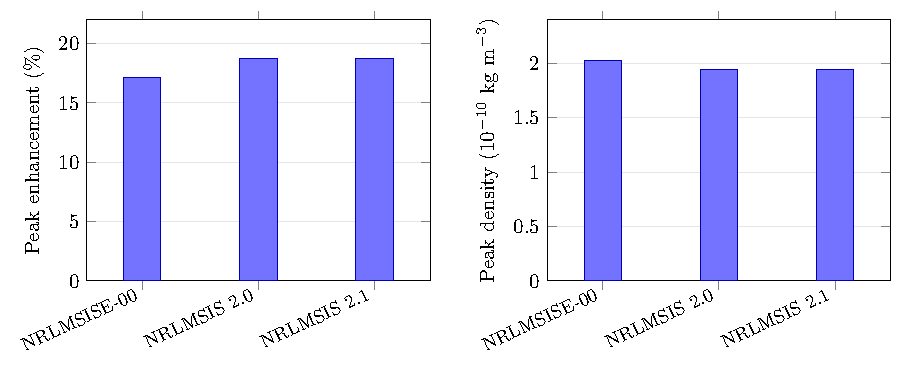
\includegraphics[width=0.80\linewidth]{figures/atmosphere_models.pdf}
\caption{Peak relative enhancement against the $ap=4$ quiet counterfactual (left, in per cent) and peak absolute native mass density (right, in $10^{-10}\unit{kg\,m^{-3}}$) for the three MSIS configurations at $210\unit{km}$, $53.22\degree$\,N, $0\degree$\,E (Table~\ref{tab:atmos}).}
\label{fig:atmos}
\end{figure}

Comparing the archived WAM-IPE operational field against NRLMSISE-00 demonstrates both substantially higher physics-based storm densities and strong dependence on the quiet-baseline operator in Equation~\eqref{eq:wam-operators} (Table~\ref{tab:wam-operators}). Across all $N=180$ overlapping archive hours (1--8~February) at $210\unit{km}$, $\rho_{\mathrm{WAM}}/\rho_{\mathrm{MSISE00}}$ has median $1.60$ and range $1.26$--$2.25$ (over the 133 window hours: median $1.60$, range $1.26$--$2.16$ against NRLMSISE-00; median $1.68$, range $1.33$--$2.26$ against NRLMSIS~2.1). Under the \emph{same-UTC-hour} operator $\Delta_{\mathrm{sh}}$ ($N=156$ non-reference hours per baseline day), WAM-IPE versus NRLMSISE-00 peak enhancements at $210\unit{km}$ are $53.49\,\%$ versus $17.17\,\%$ (ratio $3.11$) against 1~February, $48.34\,\%$ versus $11.93\,\%$ (ratio $4.05$) against 2~February, and $78.27\,\%$ versus $14.51\,\%$ (ratio $5.40$) against 8~February. Across altitude against 1~February, same-UTC-hour enhancement ratios are $2.84$ ($46.02\,\%/16.21\,\%$) at $200\unit{km}$, $3.11$ at $210\unit{km}$, $3.06$ ($65.80\,\%/21.49\,\%$) at $250\unit{km}$ and $3.04$ ($85.76\,\%/28.26\,\%$) at $300\unit{km}$ (spanning $2.84$--$5.40$ across $200$--$300\unit{km}$ and all three reference days), declining to $2.29$ ($85.19\,\%/37.23\,\%$) at $350\unit{km}$ and $2.15$ ($104.26\,\%/48.58\,\%$) at $400\unit{km}$.

By contrast, replacing same-UTC-hour differencing with the \emph{whole-day-mean} operator $\Delta_{\mathrm{dm}}$ reduces the WAM-to-MSIS peak enhancement ratios at $210\unit{km}$ to $1.24$ ($37.01\,\%$ versus $29.81\,\%$), $1.61$ ($43.90\,\%$ versus $27.22\,\%$) and $1.62$ ($49.26\,\%$ versus $30.46\,\%$) on 1, 2 and 8~February, and to $1.12$--$1.62$ across $200$--$300\unit{km}$ ($1.21, 1.24, 1.13, 1.12, 1.08, 1.07$ across $200$--$400\unit{km}$ on 1~February). The physical reason is instructive: NRLMSISE-00 peaks at 14:00~UTC near the afternoon diurnal bulge at $0\degree$\,E, so dividing by a 24-hour diurnal mean aliases roughly $13$--$16$ percentage points of normal diurnal tide into NRLMSISE-00's apparent storm anomaly while lowering WAM-IPE's 22:00~UTC nightside ratio, proving directly why storm enhancement ratios are inseparable from their diurnal baseline operator.

\begin{table}[htbp]
\centering
\footnotesize
\setlength{\tabcolsep}{4.5pt}
\caption{Sensitivity of WAM-IPE versus NRLMSISE-00 storm comparisons to reference-day baseline operator at $210\unit{km}$, $53.22\degree$\,N, $0\degree$\,E ($N=156$ evaluation hours per 24-hour reference day) and to path-quadrature support along the $96\unit{h}$ drag-free planned orbit ($\gamma = 0.026246\unit{m^2\,kg^{-1}}$).}
\label{tab:wam-operators}
\begin{tabular}{lrrrrrr}
\toprule
\multicolumn{7}{l}{\textbf{A. Fixed-point $210\unit{km}$ peak enhancements by baseline operator}} \\
\midrule
 & \multicolumn{3}{c}{same-UTC-hour $\Delta_{\mathrm{sh}}$} & \multicolumn{3}{c}{whole-day mean $\Delta_{\mathrm{dm}}$} \\
\cmidrule(lr){2-4}\cmidrule(lr){5-7}
reference day & WAM (\%) & MSIS (\%) & ratio & WAM (\%) & MSIS (\%) & ratio \\
\midrule
2022-02-01 & $53.49$ & $17.17$ & $3.11$ & $37.01$ & $29.81$ & $1.24$ \\
2022-02-02 & $48.34$ & $11.93$ & $4.05$ & $43.90$ & $27.22$ & $1.61$ \\
2022-02-08 & $78.27$ & $14.51$ & $5.40$ & $49.26$ & $30.46$ & $1.62$ \\
\midrule
\multicolumn{7}{l}{\textbf{B. Specific path-energy integrals along $96\unit{h}$ planned orbit ($\mathrm{J\,kg^{-1}}$)}} \\
\midrule
quadrature support \& metric & MSIS quiet & MSIS storm & WAM storm & \multicolumn{2}{r}{MSIS S/Q} & WAM/MSIS \\
\midrule
bridged ($985$ pts), $|\Delta E_{\mathrm{orb}}|$ & $99\,119.5$ & $109\,526.4$ & $163\,733.8$ & \multicolumn{2}{r}{$+10.50\,\%$} & $+49.49\,\%$ \\
bridged ($985$ pts), $E_{\mathrm{diss}}$ & $95\,606.0$ & $105\,642.2$ & $157\,912.1$ & \multicolumn{2}{r}{$+10.50\,\%$} & $+49.48\,\%$ \\
contiguous (3 segs), $|\Delta E_{\mathrm{orb}}|$ & $94\,564.4$ & $104\,558.3$ & $155\,160.6$ & \multicolumn{2}{r}{$+10.57\,\%$} & $+48.40\,\%$ \\
contiguous (3 segs), $E_{\mathrm{diss}}$ & $91\,219.3$ & $100\,857.7$ & $149\,655.6$ & \multicolumn{2}{r}{$+10.57\,\%$} & $+48.38\,\%$ \\
\bottomrule
\end{tabular}
\end{table}

Panel~B of Table~\ref{tab:wam-operators} resolves both path-energy observables and archive-gap sensitivity along the $96\unit{h}$ planned orbit. Because co-rotation lowers $V_{\mathrm{rel}}$ relative to inertial speed $|\mathbf{v}|$ at $53.22\degree$ prograde inclination, atmosphere-relative dissipation $E_{\mathrm{diss}}$ is uniformly $3.55\,\%$ smaller than inertial orbital-energy loss $|\Delta E_{\mathrm{orb}}|$ across every branch, yet their relative model contrasts agree to two hundredths of a percentage point ($+49.49\,\%$ versus $+49.48\,\%$ for WAM over MSIS storm, and $+10.50\,\%$ for MSIS storm over quiet on the endpoint-bridged $985$-sample grid). Excluding the two $425\unit{min}$ gap-bridging trapezoids and summing strictly over the three contiguous $5\unit{min}$ segments ($463$, $492$ and $30$ samples, where individual segment WAM/MSIS excesses are $+53.78\,\%$, $+43.44\,\%$ and $+41.62\,\%$) yields $+48.40\,\%$ ($|\Delta E_{\mathrm{orb}}|$) and $+48.38\,\%$ ($E_{\mathrm{diss}}$) for WAM over MSIS storm, and $+10.57\,\%$ for MSIS storm over quiet, confirming that the $\sim48$--$49.5\,\%$ cumulative excess is robust to gap exclusion while reflecting only covered sub-intervals.

\subsection{Panel-visibility discontinuities at $30\degree$ and exact grazing ($0\degree$)}
\label{sec:shadow}

Before interpreting paired orbital crossing times, two distinct geometric artifacts of the legacy binary centroid-ray visibility mask (\texttt{V1}) must be identified. First, at nominal $30\degree$ pitch, the solar array ($z = +1.0\unit{m}$) overhangs the $2.8\unit{m}$ bus top ($z = +0.1\unit{m}$) across vertical gap $\Delta z = 0.9\unit{m}$, leaving a collimated windward illuminated fraction $0.9\cot(30\degree)/2.8 = 0.55673$, whereas the bus-top centroid ray misses the array ($\chi_f = 1$) up to $\arctan(0.9/1.4) = 32.74\degree$. At the rounded 2022-02-04 14:00~UTC diagnostic state ($T_\infty = 923.98\unit{K}$, $V_{\mathrm{rel}} = 7495.2\unit{m\,s^{-1}}$), continuous collimated area weighting (\texttt{V2}) reduces $30\degree$ drag by $-6.48\,\%$ ($0.142048\unit{N}$ versus $0.151890\unit{N}$, matching a $128\times128$ midpoint quadrature $0.142002\unit{N}$ to $0.03194\,\%$) and replaces the $-12.26\,\%$ centroid drop between $32\degree$ and $33\degree$ ($0.161037\unit{N}$ to $0.141296\unit{N}$) with a smooth rise ($0.149589\unit{N}$ to $0.153300\unit{N}$).

Second, and equally consequential for edge-on flight, \texttt{V1} exhibits an isolated $+14.45\,\%$ discontinuity immediately above exact $0\degree$ pitch. At $\theta = 0\degree$, casting centroid rays from the four grazing bus side and top/bottom faces ($\pm y, \pm z$) with an upstream origin shift along $+\hat{\mathbf{u}}$ rather than outward normal $\hat{\mathbf{n}}_f$ strikes the perimeter boundary of the forward $+x$ bus cap, masking all four bus faces ($0.018753\unit{N}$, $\gamma = 0.011572\unit{m^2\,kg^{-1}}$). Perturbing pitch to $10^{-5}\degree$ unmasks the windward $+z$ bus top and retains the leeward $-z$ bus bottom, jumping drag by $+14.45\,\%$ to $0.021462\unit{N}$ ($\gamma = 0.013244\unit{m^2\,kg^{-1}}$), whereas both continuous collimated area (\texttt{V2}: $0.021849\unit{N}$, $\gamma = 0.013483\unit{m^2\,kg^{-1}}$) and exact parallel-plate 3D Gaussian kinetic velocity-space cavity shadowing (\texttt{V3-pair}: $0.021849\unit{N}$, $\gamma = 0.013482\unit{m^2\,kg^{-1}}$, Companion Paper~III) are smooth across $0\degree \to 10^{-5}\degree$ to $2.10\times10^{-10}\,\%$.

\subsection{Paired orbital threshold-crossing sensitivity and visibility/Knudsen checks}
\label{sec:res-orbit}

Table~\ref{tab:lifetimes} and Figure~\ref{fig:lifetimes} present the primary historical paired propagations under NRLMSIS~2.1 and \texttt{V1} centroid shadowing to first descending crossing of $170\unit{km}$ geodetic altitude ($\Delta t = t_{\mathrm{quiet}} - t_{\mathrm{observed}} > 0$ denotes earlier arrival under observed storm drivers). Observed geomagnetic drivers advance the $170\unit{km}$ crossing by $5.94\unit{h}$ ($11.77\,\%$, $0.2476\unit{d}$) at $30\degree$ pitch, by $3.04\unit{h}$ ($10.25\,\%$, $0.1265\unit{d}$) broadside ($90\degree$), and by $29.71\unit{h}$ ($6.69\,\%$) at exact $0\degree$ edge-on; continuing below $170\unit{km}$ to $100\unit{km}$ adds $6.7\,\%$ to $9.6\,\%$ of the $170\unit{km}$ elapsed time. Tightened solver checks ($30\unit{s}$ maximum step) shift crossing times and differences by at most $0.088733\unit{s}$ and $0.089632\unit{s}$, with root residuals $\le 1.863\times10^{-9}\unit{m}$ and minimum prior-perigee clearance $314.18\unit{m}$.

\begin{table}[htbp]
\centering
\small
\caption{Paired quiet-versus-storm times to first crossing of $170\unit{km}$ geodetic altitude under NRLMSIS~2.1 and historical centroid visibility (\texttt{V1}). Both day columns are modelled counterfactual branches ($ap=4$ versus observed $ap$), never observed satellite lifetimes; hour and percentage advances are computed from unrounded crossing times.}
\label{tab:lifetimes}
\begin{tabular}{lrrrrrr}
\toprule
& \multicolumn{4}{c}{first crossing of $170\,$km} & \multicolumn{2}{c}{extrapolated to $100\,$km} \\
\cmidrule(lr){2-5}\cmidrule(lr){6-7}
prescribed attitude & quiet- & observed- & diff. & diff. & quiet- & observed- \\
 & driver (d) & driver (d) & (h) & (\%) & driver (d) & driver (d) \\
\midrule
edge-on ($0\degree$, \texttt{V1} mask) & $18.511$ & $17.273$ & $29.71$ & $6.69$ & $19.965$ & $18.751$ \\
nominal, $30\degree$ (\texttt{V1} mask) & $2.103$ & $1.855$ & $5.94$ & $11.77$ & $2.283$ & $2.033$ \\
broadside ($90\degree$, \texttt{V1} mask) & $1.234$ & $1.108$ & $3.04$ & $10.25$ & $1.333$ & $1.182$ \\
\bottomrule
\end{tabular}
\end{table}

\begin{figure}[htbp]
\centering
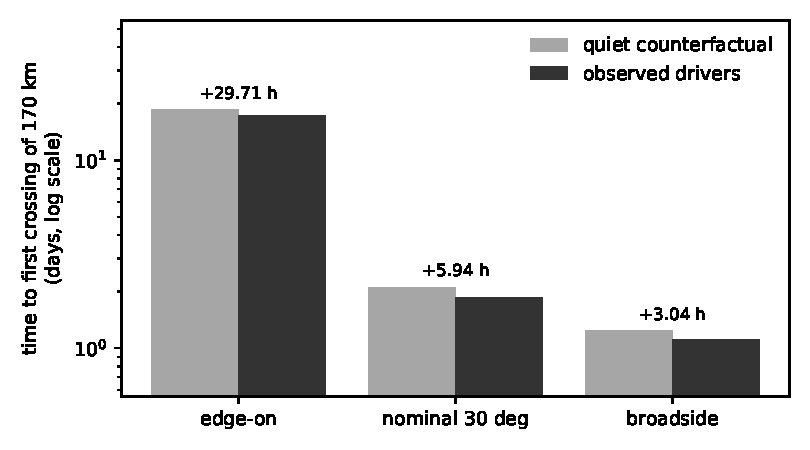
\includegraphics[width=0.72\linewidth]{figures/paired_lifetimes.pdf}
\caption{Modelled time to first crossing of $170\unit{km}$ geodetic altitude under the $ap=4$ quiet counterfactual and observed geomagnetic drivers across the three NRLMSIS~2.1 \texttt{V1} scenarios (Table~\ref{tab:lifetimes}).}
\label{fig:lifetimes}
\end{figure}

To quantify directly how the exact-grazing $+14.45\,\%$ discontinuity and $30\degree$ $-6.48\,\%$ area shadow propagate into orbital crossing times without linear drag scaling, we executed twenty fresh \texttt{DOP853} trajectories (ten quiet/storm pairs) under deterministic in-repo NRLMSISE-00 comparing \texttt{V1}, \texttt{V2} and full-vector parallel-plate kinetic cavity shadowing (\texttt{V3-pair}) at $0\degree$, $30\degree$ and $90\degree$ pitch (Table~\ref{tab:visibility-orbital}; external NRLMSIS~2.1 was not re-propagated under \texttt{V2}/\texttt{V3-pair}). For \texttt{V3-pair}, the incoming cavity moments depend solely on speed ratio $s_j$ at fixed pitch $\theta$ and are evaluated through a 120-point log-$s$ cubic spline over $s \in [0.25, 30.0]$ paired with exact runtime diffuse wall recoil $r_j(s_j, T_w/T_\infty)$, retaining \emph{both} drag and normal/lift vector components on the bus-top and array-underside facets. Runtime speed ratios remain strictly within $[1.70, 29.09]$ (zero clamping). On a dense 101-temperature test grid spanning $550$--$1400\unit{K}$ at fixed diagnostic velocity ($7495.2\unit{m\,s^{-1}}$) and peak-state composition (a finite-grid check rather than a continuum bound), the maximum observed full-vector relative error against direct adaptive quadrature is $3.95\times10^{-9}$ at $0\degree$ ($1323.5\unit{K}$), $2.67\times10^{-10}$ at $30\degree$ ($1043\unit{K}$) and $2.73\times10^{-11}$ at $90\degree$ ($1323.5\unit{K}$), with net $0\degree$ normal force $-2.10\times10^{-19}\unit{N}$ direct versus $-3.07\times10^{-12}\unit{N}$ from the spline. Twelve explicit $30\unit{s}$ maximum-step convergence checks covering quiet and storm \texttt{V2} and \texttt{V3-pair} pairs at $0\degree$, $30\degree$ and $90\degree$ shift $170\unit{km}$ crossings by at most $0.234\unit{s}$ ($0.076\unit{s}$ for $90\degree$ \texttt{V2} storm and $0.040\unit{s}$ for $90\degree$ \texttt{V3-pair} storm) and storm advances by at most $0.143\unit{s}$.

Four physical findings follow:

\begin{enumerate}
\item \textbf{Resolving the $0\degree$ centroid-mask defect shortens edge-on crossings by $2.54\unit{d}$ ($15.1\,\%$ quiet; $2.48\unit{d}$, $15.8\,\%$ storm) and reduces storm advance by $1.50\unit{h}$.} Under NRLMSISE-00, perturbing \texttt{V1} from $0\degree$ to $0.001\degree$ shifts quiet/storm crossings from $16.780/15.664\unit{d}$ (advance $26.79\unit{h}$, $6.65\,\%$) to $14.491/13.437\unit{d}$ ($25.31\unit{h}$, $7.28\,\%$). Unmasking exterior grazing faces under \texttt{V2} and full-vector \texttt{V3-pair} yields nearly identical crossings: $14.24222/13.18874\unit{d}$ ($25.2835\unit{h}$, $7.40\,\%$) versus $14.24223/13.18876\unit{d}$ ($25.2834\unit{h}$, $7.40\,\%$), agreeing within $2\unit{s}$ ($1.23\unit{s}$ quiet, $1.54\unit{s}$ storm) in crossing time and $0.31\unit{s}$ ($0.30\unit{s}$) in storm advance. Equivalently, legacy \texttt{V1} inflates $0\degree$ quiet crossings by $+17.8\,\%$ relative to \texttt{V2}/\texttt{V3-pair}.

\item \textbf{At $30\degree$ pitch, both \texttt{V2} and full-vector \texttt{V3-pair} lengthen crossing times by $6.3\,\%$--$7.1\,\%$ while shifting storm advance by under $1.7\unit{min}$.} Replacing \texttt{V1} ($1.979/1.732\unit{d}$, advance $5.927\unit{h}$, $12.48\,\%$) with \texttt{V2} ($2.10361/1.85552\unit{d}$, $5.954\unit{h}$, $11.79\,\%$) or executed \texttt{V3-pair} ($2.10362/1.85553\unit{d}$, $5.954\unit{h}$, $11.79\,\%$) increases advance by $1.623\unit{min}$, with \texttt{V2} and \texttt{V3-pair} matching to $0.85\unit{s}$ ($0.006\unit{s}$ in advance).

\item \textbf{At $90\degree$ broadside, \texttt{V1}, \texttt{V2} and \texttt{V3-pair} are distinct, and perigee-pass quantisation amplifies \texttt{V3-pair}'s $+0.35\,\%$ kinetic drag increment into a one-orbit threshold step.} Unmasking the four grazing bus walls in \texttt{V2} raises broadside static drag by $+0.22\,\%$ above \texttt{V1} ($0.262075\unit{N}$ vs $0.261494\unit{N}$; Companion Paper~III), shifting crossings smoothly on the same perigee pass by $-25.1\unit{s}$ quiet and $-25.6\unit{s}$ storm ($1.171/1.045\unit{d}$ vs $1.171/1.046\unit{d}$, both giving $3.02\unit{h}$ / $10.74\,\%$ advance; $100\unit{km}$ storm descent $-2.84\unit{min}$ from $1.114\unit{d}$ to $1.112\unit{d}$). Lateral thermal spillover in \texttt{V3-pair} raises broadside drag by a further $+0.35\,\%$ above \texttt{V2} ($+0.58\,\%$ above \texttt{V1}, to $0.263002\unit{N}$), tipping the near-tangent storm perigee pass across $170\unit{km}$ one revolution ($\sim78\unit{min}$) earlier ($1.171/0.991\unit{d}$, advance $4.31\unit{h}$, $15.35\,\%$, stable to $0.040\unit{s}$ at $30\unit{s}$ maximum step), while continuous $100\unit{km}$ storm descent shifts smoothly by $-4.34\unit{min}$ relative to \texttt{V2} ($1.112\unit{d} \to 1.109\unit{d}$, or $-7.18\unit{min}$ relative to \texttt{V1}; $100\unit{km}$ advance $3.47\unit{h} \to 3.44\unit{h}$).

\item \textbf{Accepted dense-output pre-$t_{170}$ Knudsen samples remain $>10$ across all $0\degree$ and $30\degree$ arcs while showing broadside storm dips to $\mathrm{Kn} = 9.32$--$9.33$.} We sample accepted dense-output trajectory states over $t \le t_{170}$ at spacing $\le 30\unit{s}$ plus accepted solver knots ($4\,291$--$72\,496$ samples per trajectory, excluding solver trial stages and post-$t_{170}$ points; this is not a continuous lower-bound proof between samples). At worst-case $d = 3.64\,\text{\normalfont\AA}$ and $L = 8.0\unit{m}$, every $0\degree$ and $30\degree$ trajectory yields sampled $\min\mathrm{Kn} \ge 10.31$ ($10.31$--$11.42$). By contrast, $90\degree$ \texttt{V1} and \texttt{V2} storm trajectories dip to $\mathrm{Kn} = 9.32$ and $9.33$ at $t_{170} = 1.046$ and $1.045\unit{d}$ ($170.00\unit{km}$; $> 26$ on the $2.8\unit{m}$ array chord), while $90\degree$ \texttt{V3-pair} storm crosses one orbit earlier with sampled minimum $\mathrm{Kn} = 10.55$.
\end{enumerate}

\begin{table}[htbp]
\centering
\footnotesize
\setlength{\tabcolsep}{4.5pt}
\caption{Paired \texttt{DOP853} threshold-crossing and accepted dense-output sampled minimum Knudsen-number sensitivity ($\le 30\unit{s}$ spacing plus solver knots over $t \le t_{170}$, $d=3.64\,\text{\normalfont\AA}$, $L=8.0\unit{m}$) across panel-visibility formulations under deterministic NRLMSISE-00.}
\label{tab:visibility-orbital}
\begin{tabular}{llrrrrrr}
\toprule
pitch & visibility & quiet & storm & advance & advance & \multicolumn{2}{c}{sampled $\min_{t\le t_{170}}\mathrm{Kn}$} \\
\cmidrule(lr){7-8}
($\degree$) & model & $170\,$km (d) & $170\,$km (d) & (h) & (\%) & quiet & storm \\
\midrule
$0$ & \texttt{V1} legacy centroid & $16.780$ & $15.664$ & $26.79$ & $6.65$ & $10.42$ & $10.59$ \\
$0.001$ & \texttt{V1} legacy centroid & $14.491$ & $13.437$ & $25.31$ & $7.28$ & $11.42$ & $11.16$ \\
$0$ & \texttt{V2} collimated area & $14.242$ & $13.189$ & $25.28$ & $7.40$ & $11.22$ & $10.90$ \\
$0$ & \texttt{V3-pair} full-vector & $14.242$ & $13.189$ & $25.28$ & $7.40$ & $11.22$ & $10.90$ \\
$30$ & \texttt{V1} legacy centroid & $1.979$ & $1.732$ & $5.93$ & $12.48$ & $10.84$ & $10.57$ \\
$30$ & \texttt{V2} collimated area & $2.104$ & $1.856$ & $5.95$ & $11.79$ & $11.01$ & $10.31$ \\
$30$ & \texttt{V3-pair} full-vector & $2.104$ & $1.856$ & $5.95$ & $11.79$ & $11.01$ & $10.31$ \\
$90$ & \texttt{V1} legacy centroid & $1.171$ & $1.046$ & $3.02$ & $10.74$ & $10.42$ & $9.32$ \\
$90$ & \texttt{V2} collimated area & $1.171$ & $1.045$ & $3.02$ & $10.74$ & $10.40$ & $9.33$ \\
$90$ & \texttt{V3-pair} full-vector & $1.171$ & $0.991$ & $4.31$ & $15.35$ & $10.38$ & $10.55$ \\
\bottomrule
\end{tabular}
\end{table}

Crucially, even after repairing the $0\degree$ mask (\texttt{V2}/\texttt{V3-pair}), the multi-week edge-on pair and the one-to-two-day inclined pairs do not isolate the same geomagnetic interval. In Table~\ref{tab:lifetimes}, broadside and $30\degree$ observed crossings occur at \texttt{2022-02-04 21:03:04 UTC} and \texttt{2022-02-05 14:59:33 UTC} ($29.53$ of $44.53\unit{h}$ inside 3--4~February), whereas edge-on trajectories cross $170\unit{km}$ between 16 and 22~February across subsequent disturbances on 10--13~February ($ap$ up to $48$) and 20--21~February ($ap$ up to $39$).

\section{Discussion and Limitations}
\label{sec:discussion}

\subsection{Synthesis of atmospheric operators and propagated contrasts}
\label{sec:synthesis}

Taken together, the fixed-point atmospheric series, dual-operator WAM-IPE comparisons and visibility-resolved paired propagations demonstrate why forward space-weather metrics must be interpreted strictly through their mathematical operators. Within the MSIS lineage at $210\unit{km}$, changing generation from NRLMSISE-00 to NRLMSIS~2.0/2.1 alters the $ap=4$ peak enhancement by $1.63$ percentage points ($17.14\,\%$ to $18.77\,\%$), whereas sweeping the quiet counterfactual across $ap=2$--$7$ spans $7.40$ percentage points ($20.58\,\%$ to $13.18\,\%$). Against archived WAM-IPE fields across $200$--$300\unit{km}$, controlling for diurnal phase via same-UTC-hour baselines yields WAM-to-MSIS peak enhancement ratios of $2.84$ to $5.40$, whereas whole-day reference means compress those ratios to $1.12$--$1.62$ by mixing diurnal tide into the denominator; along the $96\unit{h}$ planned orbit, WAM-IPE increases orbital-energy loss and co-rotating dissipation by $49.5\,\%$ ($48.4\,\%$ over contiguous non-gap support).

Across all paired orbital propagations under both NRLMSIS~2.1 and NRLMSISE-00, observed geomagnetic drivers advance $170\unit{km}$ crossings consistently by $3.02$--$4.31\unit{h}$ broadside (the upper value reflecting a single perigee-pass threshold step under \texttt{V3-pair}), $5.93$--$5.95\unit{h}$ at $30\degree$ pitch (comparable in magnitude to the $\sim6\unit{h}$ JB2008 / $1\unit{m^2}$ result of \citet{baruah2024}, while resolving attitude, atmospheric-operator and panel-shadowing dependence explicitly) and $25.28$--$29.71\unit{h}$ edge-on. Replacing binary centroid visibility (\texttt{V1}) with continuous collimated area (\texttt{V2}) or full-vector parallel-plate kinetic cavity shadowing (\texttt{V3-pair}) leaves the $30\degree$ storm advance virtually unchanged ($5.93\unit{h}$ to $5.95\unit{h}$, with \texttt{V2} and \texttt{V3-pair} agreeing to $0.85\unit{s}$) while correcting \texttt{V1}'s $+2.54\unit{d}$ ($+17.8\,\%$) edge-on crossing-time inflation and $+1.50\unit{h}$ advance inflation ($0\degree$ \texttt{V2} and \texttt{V3-pair} agree within $2\unit{s}$). None of these dimensionless percentage and ratio contrasts --- $6.65$--$12.48\,\%$ crossing advances ($15.35\,\%$ across the $90\degree$ \texttt{V3-pair} perigee-pass step), $17.14$--$18.77\,\%$ MSIS storm peaks, the $10.26\,\%$ single-state molecular-over-scalar force offset, and the $12.04\times$ parallel-cavity ($12.02\times$ full-polyhedral, $13.94\times$ legacy) single-state attitude span in Companion Paper~III --- may be combined or ranked as competing error budgets, because they act on different observables, operators, baselines and denominators. Nor can public satellite-catalogue decay dates validate the short-pair $3$--$6\unit{h}$ advances against $\pm12\unit{h}$ calendar-date rounding and payload/debris pooling (Companion Paper~II).

\subsection{Physical, geometric and observational limitations}
\label{sec:limits}

Every trajectory starts from a single planned state ($\Omega=\omega=\nu=0\degree$) with constant ram-frame pitch, zero neutral wind, fixed wall temperature ($300\unit{K}$), fixed accommodation ($\alpha=0.998$), idealized proxy dimensions and $297\unit{kg}$ mass. Companion Paper~II shows that same-orbit $J_2$-transported phase shifts alter scalar decay fits by only $0.23\,\%$ whereas non-constant-shape osculating and $E$-matched conventions span $15.85\,\%$--$44.29\,\%$, and Companion Paper~III shows that Cercignani--Lampis--Lord scattering spans $-36.1\,\%$ to $+6.8\,\%$ in single-state drag. Those sensitivities have not yet been propagated through facet-resolved paired ensembles, and visibility-corrected \texttt{V2}/\texttt{V3-pair} trajectories were executed under NRLMSISE-00 rather than external licensed NRLMSIS~2.1. Moreover, free-streaming panel summation omits secondary inter-panel reflections inside the bus--array gap and full-8-facet polyhedral occlusion on the lateral bus walls ($-4.01\times10^{-5}\,\%$ at $0\degree$ to $-0.144\,\%$ at $90\degree$ in single-state drag, Companion Paper~III). Finally, observations at $438$--$505\unit{km}$ do not adjudicate model bias at $210\unit{km}$, coupled attitude/propulsion dynamics are unmodelled, and transitional flow below $170\unit{km}$ ($155$--$190\unit{km}$ across cross-section brackets, with broadside \texttt{V1} and \texttt{V2} storm dips to $\mathrm{Kn} = 9.32$ and $9.33$ at $170.00\unit{km}$) requires rarefied-gas kinetic solvers.

\section{Conclusion}
\label{sec:conclusions}

Forward thermospheric evaluations and paired free-molecular orbital propagations for the February 2022 Starlink Group~4-7 deployment establish four bounded conclusions.

\begin{enumerate}
\item At $210\unit{km}$, $53.22\degree$\,N, $0\degree$\,E, NRLMSISE-00 and NRLMSIS~2.0/2.1 yield actual-to-quiet peak enhancements of $17.14\,\%$ and $18.77\,\%$ against $ap=4$ ($20.58\,\%$ to $13.18\,\%$ across $ap=2$--$7$ on NRLMSISE-00). Across $200$--$300\unit{km}$, fixed-point WAM-IPE to NRLMSISE-00 ratios of independently maximised storm-time peak percentage enhancements span $2.84$ to $5.40$ under same-UTC-hour reference-day baselines versus $1.12$ to $1.62$ under whole-day means. These ratios compare non-simultaneous percentage peaks rather than simultaneous absolute densities: at $210\unit{km}$ under the 1~February same-UTC-hour baseline, the $53.49\,\%$ and $17.17\,\%$ peaks occur $2\unit{h}$ apart, versus a $1.60$ median matched-hour absolute density ratio over 180 hours. Separately, along the $96\unit{h}$ planned orbit, WAM-IPE increases orbital-energy loss and co-rotating dissipation by $49.5\,\%$ ($48.4\,\%$ over contiguous non-gap segments).

\item Differences in reference baseline, spatial averaging and altitude prevent direct numerical ranking against published storm enhancements, and satellite density observations near $438$--$505\unit{km}$ do not certify model accuracy at $210\unit{km}$.

\item Under NRLMSIS~2.1 and historical centroid visibility (\texttt{V1}), observed geomagnetic drivers advance first crossing of $170\unit{km}$ geodetic altitude by $5.94\unit{h}$ ($11.77\,\%$) at $30\degree$ pitch, $3.04\unit{h}$ ($10.25\,\%$) broadside and $29.71\unit{h}$ ($6.69\,\%$) edge-on across multi-week disturbances.

\item Full-vector paired NRLMSISE-00 propagations (twenty trajectories across ten pairs, with twelve $30\unit{s}$ step checks across $0\degree$, $30\degree$ and $90\degree$ verified to $\le 0.234\unit{s}$) show that replacing discontinuous centroid visibility (\texttt{V1}) with continuous collimated area (\texttt{V2}) or parallel-plate kinetic cavity shadowing (\texttt{V3-pair}) keeps $30\degree$ storm advance at $5.95\unit{h}$ ($11.79\,\%$; \texttt{V2} and \texttt{V3-pair} agree to $0.85\unit{s}$). Edge-on crossings shorten by $2.54\unit{d}$ ($15.1\,\%$ quiet; $15.8\,\%$ storm), shifting edge-on storm advance from $26.79\unit{h}$ ($6.65\,\%$) to $25.28\unit{h}$ ($7.40\,\%$; \texttt{V2} and \texttt{V3-pair} agree within $2\unit{s}$); at $90\degree$, \texttt{V2} shifts smoothly by $-25.6\unit{s}$ relative to \texttt{V1} while \texttt{V3-pair} tips across $170\unit{km}$ one orbit earlier ($4.31\unit{h}$ advance). Accepted dense-output pre-$t_{170}$ Knudsen samples ($\le 30\unit{s}$ spacing plus solver knots) stay $\ge 10.31$ across all $0\degree$ and $30\degree$ runs and dip to $9.32$ and $9.33$ on $90\degree$ \texttt{V1} and \texttt{V2} storm runs.
\end{enumerate}

\section{Data and Code Availability}
\label{sec:availability}

\begin{sloppypar}All open-source Apache-2.0 Python simulation modules (\nolinkurl{src/thermosphere_consequence/}), deterministic reproduction scripts (\texttt{scripts/}, including \nolinkurl{run_referee_revision_diagnostics.py}, \nolinkurl{run_atmosphere_audit.py} and \nolinkurl{reproduce_paired_lifetimes_public.py}), portable dependency specification (\texttt{requirements.portable.txt}), configuration files and derived JSON/CSV summary tables are archived in the standalone release repository \nolinkurl{waynestark-starlink-thermosphere-orbital-decay} (\url{https://github.com/wseltd/waynestark-starlink-thermosphere-orbital-decay}, release \texttt{v1.0.0}; archival Zenodo DOI assigned upon public release). The repository also includes a cryptographic SHA-256 manifest (\texttt{MANIFEST.sha256}), shared-kernel provenance (\nolinkurl{KERNEL_PROVENANCE.json}) and an offline/live verification runner (\nolinkurl{verify_all_claims.py}). External geomagnetic and solar-flux drivers from GFZ Potsdam (CC~BY~4.0) and CelesTrak, together with the 180 NOAA SWPC WAM-IPE fixed-height NetCDF slices from NASA GSFC CCMC (\texttt{WAM-IPE-July2021-22}), are publicly accessible from their upstream archives and SHA-256-pinned in \nolinkurl{evidence/DATA_MANIFEST_PAPER1.json}. Official NRLMSIS~2.0 and~2.1 Fortran source packages carry academic/non-commercial US Naval Research Laboratory licences prohibiting third-party redistribution and must be obtained directly from NRL following \texttt{README.md} and \nolinkurl{third_party/nrlmsis_asset_manifest.yaml}, whereas NRLMSISE-00 runs directly via \texttt{pymsis==0.12.0}. The author thanks the U.S. Naval Research Laboratory Technology Transfer and Patent Offices for written confirmation permitting open, non-commercial scientific research use of NRLMSIS~2.0 and~2.1 under their academic research licences; MSIS\textsuperscript{\textregistered} is a registered trademark of the U.S. Government. Software and manuscript preparation used AI coding and editorial assistants under the author's direction; all scientific judgements and responsibility rest with the author.\end{sloppypar}

\begin{thebibliography}{20}
\providecommand{\natexlab}[1]{#1}
\providecommand{\url}[1]{\texttt{#1}}
\expandafter\ifx\csname urlstyle\endcsname\relax
  \providecommand{\doi}[1]{doi: #1}\else
  \providecommand{\doi}{doi: \begingroup \urlstyle{rm}\Url}\fi

\bibitem[Baruah et~al.(2024)Baruah, Roy, Sinha, Palmerio, Pal, Oliveira, and
  Nandy]{baruah2024}
Yoshita Baruah, Souvik Roy, Suvadip Sinha, Erika Palmerio, Sanchita Pal,
  Denny~M. Oliveira, and Dibyendu Nandy.
\newblock The loss of {Starlink} satellites in {February} 2022: How moderate
  geomagnetic storms can adversely affect assets in low-{Earth} orbit.
\newblock \emph{Space Weather}, 22\penalty0 (4):\penalty0 e2023SW003716, 2024.
\newblock \doi{10.1029/2023SW003716}.

\bibitem[{CCMC}(2026)]{ccmcwamipe}
{Community Coordinated Modeling Center (CCMC)}.
\newblock {WAM-IPE} Forecast System (WFS) operational run for {NOAA} {SWPC},
  July 2021--2022: fixed-height postprocessed neutral density (\texttt{WAM-IPE-July2021-22}), 2026.
\newblock URL \url{https://ccmc.gsfc.nasa.gov/}.

\bibitem[{CelesTrak}(2026)]{celestrak}
{CelesTrak}.
\newblock Daily space-weather data file (\texttt{SW-Last5Years.csv}), 2026.
\newblock URL \url{https://celestrak.org/SpaceData/SW-Last5Years.csv}.

\bibitem[Emmert et~al.(2021)]{emmert2021}
J.~T. Emmert, D.~P. Drob, J.~M. Picone, D.~E. Siskind, M.~Jones~Jr., M.~G.
  Mlynczak, et~al.
\newblock {NRLMSIS} 2.0: A whole-atmosphere empirical model of temperature and
  neutral species densities.
\newblock \emph{Earth and Space Science}, 8\penalty0 (3):\penalty0
  e2020EA001321, 2021.
\newblock \doi{10.1029/2020EA001321}.

\bibitem[Emmert et~al.(2022)]{emmert2022}
J.~T. Emmert, M.~Jones~Jr., D.~P. Drob, J.~M. Picone, D.~E. Siskind, M.~G.
  Mlynczak, et~al.
\newblock {NRLMSIS} 2.1: Empirical model of nitric oxide incorporated into
  {MSIS}.
\newblock \emph{Journal of Geophysical Research: Space Physics}, 127\penalty0
  (10):\penalty0 e2022JA030896, 2022.
\newblock \doi{10.1029/2022JA030896}.

\bibitem[Fang et~al.(2022)Fang, Kubaryk, Goldstein, Li, Fuller-Rowell,
  Millward, Singer, Steenburgh, Westerman, and Babcock]{fang2022}
Tzu-Wei Fang, Adam Kubaryk, David Goldstein, Zhuxiao Li, Tim Fuller-Rowell,
  George Millward, Howard~J. Singer, Robert Steenburgh, Solomon Westerman, and
  Erik Babcock.
\newblock Space weather environment during the {SpaceX} {Starlink} satellite
  loss in {February} 2022.
\newblock \emph{Space Weather}, 20\penalty0 (11):\penalty0 e2022SW003193, 2022.
\newblock \doi{10.1029/2022SW003193}.

\bibitem[{GFZ German Research Centre for Geosciences}(2026)]{gfzkp}
{GFZ German Research Centre for Geosciences}.
\newblock {$K_p$} and $ap$ geomagnetic indices (CC~BY~4.0; Matzka et~al., 2021, doi:10.5880/Kp.0001), 2026.
\newblock URL \url{https://kp.gfz.de/}.

\bibitem[Guarnieri et~al.(2023)]{guarnieri2023v1}
Fernando Guarnieri, Bruce~T. Tsurutani, Rajkumar Hajra, Ezequiel Echer, and Gurbax~S. Lakhina.
\newblock NORAD Tracking of the February 2022 Starlink Satellites (and the Possible Immediate Loss of 32 Satellites).
\newblock Preprint, arXiv:2307.02923v1, 2023.
\newblock URL \url{https://arxiv.org/abs/2307.02923v1}.

\bibitem[Guarnieri et~al.(2025)]{guarnieri2025}
F.~L. Guarnieri, B.~T. Tsurutani, R.~Hajra, E.~Echer, and G.~S. Lakhina.
\newblock NORAD tracking of the 2022 February Starlink satellites and the
  immediate loss of 32 satellites.
\newblock \emph{Nonlinear Processes in Geophysics}, 32:\penalty0 75--88, 2025.
\newblock \doi{10.5194/npg-32-75-2025}.

\bibitem[He et~al.(2023)He, Astafyeva, Yue, Pedatella, Lin, Fuller-Rowell,
  Fedrizzi, Codrescu, Doornbos, Siemes, Bruinsma, Pitout, and Kubaryk]{he2023}
Jianhui He, Elvira Astafyeva, Xinan Yue, Nicholas~M. Pedatella, Dong Lin,
  Timothy~J. Fuller-Rowell, Mariangel Fedrizzi, Mihail Codrescu, Eelco
  Doornbos, Christian Siemes, Sean Bruinsma, Frederic Pitout, and Adam Kubaryk.
\newblock Comparison of empirical and theoretical models of the thermospheric
  density enhancement during the 3--4 {February} 2022 geomagnetic storm.
\newblock \emph{Space Weather}, 21\penalty0 (9):\penalty0 e2023SW003521, 2023.
\newblock \doi{10.1029/2023SW003521}.

\bibitem[Nager et~al.(2026)Nager, Kirk, and Kilic]{nager2026}
Kylie Nager, James Kirk, and Cagri Kilic.
\newblock {HELIO}: {AI} solar weather forecasting for proactive small satellite
  constellation response.
\newblock In \emph{Proceedings of the Annual Small Satellite Conference
  (SmallSat 2026)}, Paper SSC26-P2-26, Salt Lake City, UT, August 2026.

\bibitem[Picone et~al.(2002)Picone, Hedin, Drob, and Aikin]{picone2002}
J.~M. Picone, A.~E. Hedin, D.~P. Drob, and A.~C. Aikin.
\newblock {NRLMSISE-00} empirical model of the atmosphere: Statistical
  comparisons and scientific issues.
\newblock \emph{Journal of Geophysical Research: Space Physics}, 107\penalty0
  (A12):\penalty0 1468, 2002.
\newblock \doi{10.1029/2002JA009430}.

\bibitem[Sentman(1961)]{sentman1961}
L.~H. Sentman.
\newblock Free molecule flow theory and its application to the determination of
  aerodynamic forces.
\newblock Technical Report LMSC-448514 (DTIC AD0265409), Lockheed Missiles and Space Company,
  1961.
\newblock \doi{10.21236/ad0265409}.

\bibitem[Shambaugh(2024)]{shambaugh2024}
W.~Scott Shambaugh.
\newblock Doing battle with the sun: Lessons from {LEO} and operating a
  satellite constellation in the elevated atmospheric drag environment of solar
  cycle 25.
\newblock Preprint, arXiv:2406.08342v1 (4S Symposium 2024), 2024.
\newblock URL \url{https://arxiv.org/abs/2406.08342}.

\end{thebibliography}
\end{document}
